\documentclass{article}

\usepackage{kotex}
\usepackage{amssymb}
\usepackage{graphicx}

\graphicspath{ {./images/} }

\renewcommand{\figurename}{그림}
\renewcommand{\tablename}{표}

\title{Mirésatanä 2 데이터시트}
\author{아이즌 Z. 스치 @ Lofanfashasch 1013193}

\begin{document}

\maketitle
\tableofcontents

\pagebreak

\section{부품 설계}

\subsection{ArithmetricLogicBit}

ArithmetricLogicBit는 논리곱과 배타적 논리합,
전가산 결과를 출력하는 ArithmetricLogic의 구성 부품이다.

ArithmetricLogicBit는
$A$, $B$, $C_i$, $N$, $X$의 입력 핀과
$C_o$, $O$의 출력 핀을 가지고 있고,
각각은 다음을 의미한다.

\begin{itemize}
    \item $A$ -- A. 연산의 첫 번째 인자가 될 비트
    \item $B$ -- B. 연산의 두 번째 인자가 될 비트
    \item $C_i$ -- Carry In. 이전 가산기에서 발생한 올림 비트
    \item $N$ -- aNd enable. $O$가 $A \veebar B$를 출력하게 만드는 비트
    \item $X$ -- Xor enable. $O$가 $AB$를 출력하게 만드는 비트
    \item $C_o$ -- Carry Out. 가산 연산 중 발생한 올림 비트
    \item $O$ -- Output. 연산의 결과
\end{itemize}

ArithmetricLogicBit의 진리표는 \tablename{} \ref{tab:alb}과 같이 주어진다.

\begin{table}[h]
    \centering
    \begin{tabular}{ccccc|cc}
        $A$ & $B$ & $C_i$ & $N$ & $X$ & $C_o$ & $O$ \\
        \hline
        $A$ & $B$ & $C_i$ &  0 &  0 & $AB + BC_i + C_iA$ & $A \oplus B \oplus C_i$ \\
        $A$ & $B$ & $C_i$ &  0 &  1 &  0 & $A \oplus B$ \\
        $A$ & $B$ & $C_i$ &  1 &  0 &  0 & $AB$ \\
    \end{tabular}
    \caption{ArithmetricLogicBit의 진리표}
    \label{tab:alb}
\end{table}

\figurename{} \ref{fig:alb}은 ArithmetricLogicBit의 회로도이다.

\begin{figure}[h]
    \centering
    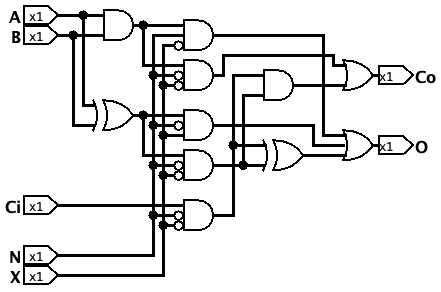
\includegraphics[scale=0.5]{ArithmetricLogicBit} \\
    \caption{ArithmetricLogicBit의 회로도}
    \label{fig:alb}
\end{figure}

\subsection{ArithmetricLogic}

ArithmetricLogic은 8비트 정수의 산술 연산과 논리 연산을 수행하는 부품이다.

ArithmetricLogic은 $A$, $B$, $I_A$, $I_B$, $I_O$, $B_e$, $N$, $X$, $C_i$의 입력 핀과
$O$, $C_o$의 출력 핀을 가지고 있다.
각각은 다음을 의미한다.

\begin{itemize}
    \item $A$ -- A. 연산의 첫 번째 인자가 될 수
    \item $B$ -- B. 연산의 두 번째 인자가 될 수
    \item $I_A$ -- Invert A. $A$의 결과를 반전하여 연산을 진행한다.
    \item $I_B$ -- Invert B. $\neg B$를 내부 두 번째 인자 입력에 논리합한다.
    \item $I_O$ -- Invert O. $O$의 결과를 반전하여 출력한다.
    \item $B_e$ -- B Enable. $B$를 내부 두 번째 인자 입력에 논리합한다.
    \item $N$ -- aNd enable. 두 수의 논리곱을 $O$에 출력한다.
    \item $X$ -- Xor enable. 두 수의 배타적 논리합을 $O$에 출력한다.
    \item $C_i$ -- Carry In. 가산 연산에 반영할 올림 비트
    \item $O$ -- Output. 연산의 결과
    \item $C_o$ -- Carry Out. 가산 연산에서 발생한 올림 비트
\end{itemize}

ArithmetricLogic은 입력되는 옵션에 따라 두 인자 $A$, $B$에 대한
$A$, $\neg A$, $A+1$, $A-1$, $A+B$, $A-B$, $-A$, $B-A$,
$A \veebar B$, $\neg(A \veebar B)$, $A\wedge B$, $\neg (A \wedge B)$, $A \vee B$, $\neg(A \vee B)$ 등을
계산할 수 있다.

ArithmetricLogic은 \tablename{} \ref{tab:al}와 같은 진리표를 가진다.
논리합($\vee$)과 산술합($+$) 연산에 주의해야 한다.

\begin{table}[p]
    \centering
    \begin{tabular}{cc|ccccccc|ll}
        $A$ & $B$ & $I_A$ & $I_B$ & $I_O$ & $B_e$ & $N$ & $X$ & $C_i$ & $O$ & $C_i$ \\
        \hline
        $A$ & $B$ & 0 & 0 & 0 & 0 & - & - & 0 & $A$ & 0 \\
        $A$ & $B$ & 0 & 0 & 0 & 0 & - & - & 1 & $A + 1$ & $\forall A$ \\
        $A$ & $B$ & 0 & 0 & 0 & 1 & 0 & 0 & 0 & $A + B$ & - \\
        $A$ & $B$ & 0 & 0 & 0 & 1 & 0 & 0 & 1 & $A + B + 1$ & - \\
        $A$ & $B$ & 0 & 0 & 0 & 1 & 0 & 1 & 0 & $A \veebar B$ & 0 \\
        $A$ & $B$ & 0 & 0 & 0 & 1 & 1 & 0 & 0 & $A \wedge B$ & 0 \\
        $A$ & $B$ & 0 & 0 & 1 & 0 & - & - & 0 & $\neg A$ & 0 \\
        $A$ & $B$ & 0 & 0 & 1 & 1 & 0 & 1 & 0 & $\neg(A \veebar B)$ & 0 \\
        $A$ & $B$ & 0 & 0 & 1 & 1 & 1 & 0 & 0 & $\neg(A \wedge B)$ & 0 \\
        $A$ & $B$ & 0 & 1 & 0 & 0 & 0 & 0 & 0 & $A - B - 1$ & $A > B$\\
        $A$ & $B$ & 0 & 1 & 0 & 0 & 0 & 0 & 1 & $A - B$ & $A \geq B$\\
        $A$ & $B$ & 0 & 1 & 0 & 1 & 0 & 0 & 0 & $A - 1$ & $\exists A$\\
        $A$ & $B$ & 0 & 1 & 1 & 0 & 0 & 0 & 0 & $B - A$ & $A > B$\\
        $A$ & $B$ & 0 & 1 & 1 & 0 & 0 & 0 & 1 & $B - A - 1$ & $A \geq B$\\
        $A$ & $B$ & 1 & 0 & 0 & 0 & 0 & 0 & 0 & $\neg A$ & 0 \\
        $A$ & $B$ & 1 & 0 & 0 & 0 & 0 & 0 & 1 & $-A$ & $\forall A$ \\
        $A$ & $B$ & 1 & 0 & 0 & 1 & 0 & 0 & 0 & $B - A - 1$ & - \\
        $A$ & $B$ & 1 & 0 & 0 & 1 & 0 & 0 & 1 & $B - A$ & - \\
        $A$ & $B$ & 1 & 1 & 0 & 0 & 0 & 0 & 0 & $-A-B-2$ & - \\
        $A$ & $B$ & 1 & 1 & 0 & 0 & 0 & 0 & 1 & $-A-B-1$ & - \\
        $A$ & $B$ & 1 & 1 & 0 & 0 & 1 & 0 & 0 & $\neg(A \vee B)$ & - \\
        $A$ & $B$ & 1 & 1 & 0 & 1 & 0 & 0 & 0 & $-A-2$ & $\neg \forall A$ \\
        $A$ & $B$ & 1 & 1 & 0 & 1 & 0 & 0 & 1 & $-A-1$ & 1 \\
        $A$ & $B$ & 1 & 1 & 1 & 0 & 1 & 0 & 0 & $A \vee B$ & 0 \\
    \end{tabular}
    \caption{ArithmetricLogic}
    \label{tab:al}
\end{table}

\figurename{} \ref{fig:al}은 ArithmetricLogic의 회로도이다.

\begin{figure}[p]
    \centering
    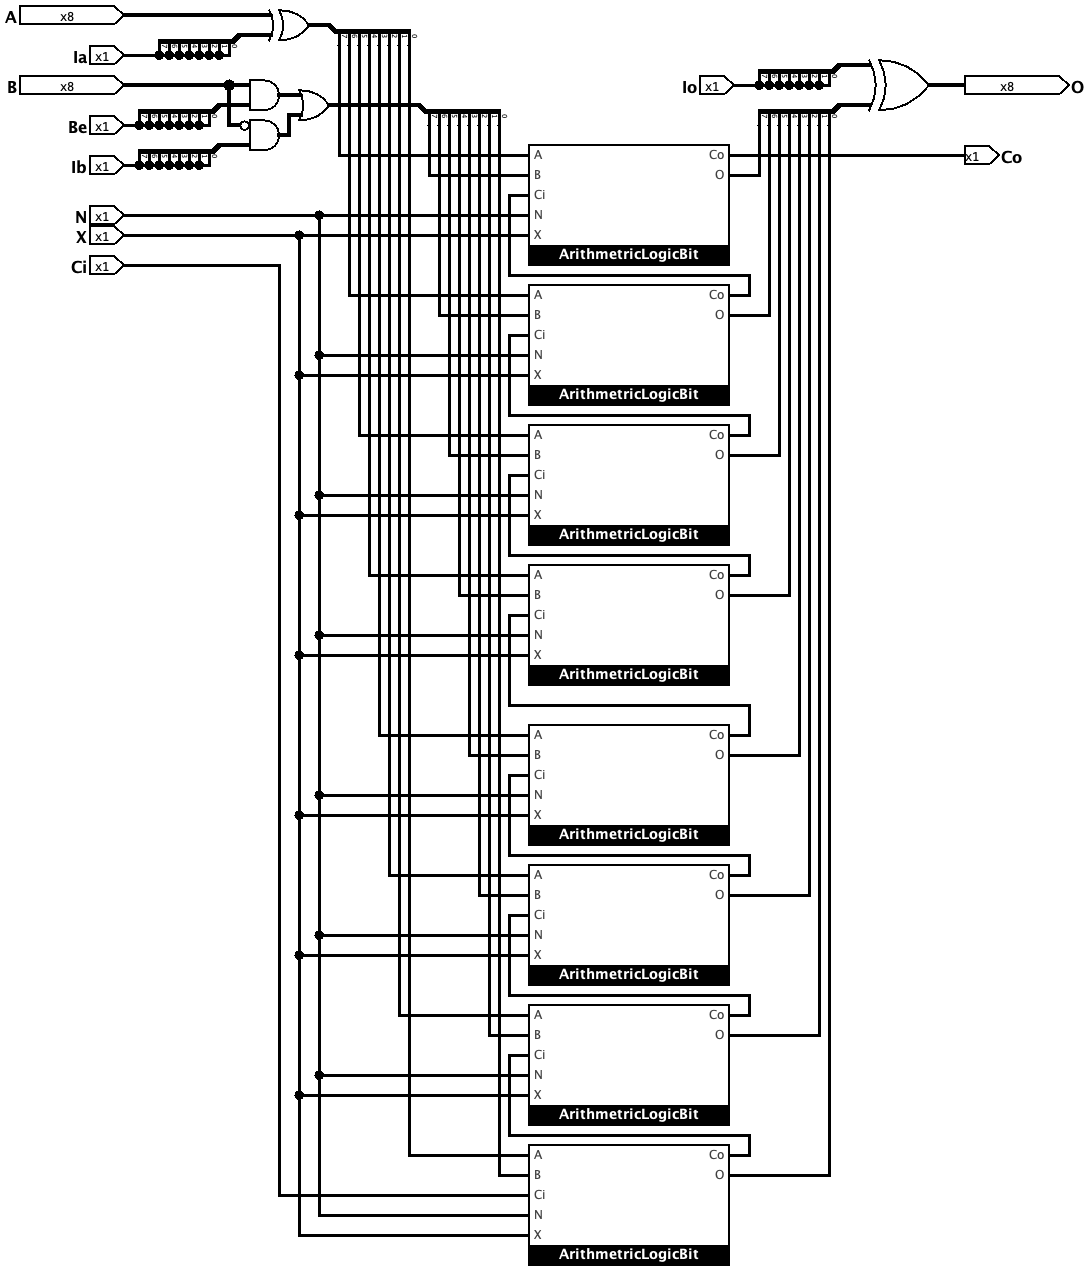
\includegraphics[scale=0.35]{ArithmetricLogic} \\
    \caption{ArithmetricLogic의 회로도}
    \label{fig:al}
\end{figure}

\pagebreak % CAUTION

\subsection{Shiftre}

Shiftre는 입력된 값에 대한 1회 좌측·우측 시프트 연산 결과를 출력하는
부품이다.

Shiftre는 $I$, $S$, $R$, $L$의 입력 핀과
$O$, $O_l$, $O_r$의 출력 핀을 가지고 있다. 각각은 다음을 의미한다.

\begin{itemize}
    \item $I$ -- Input. 시프트 연산을 수행할 정수
    \item $E$ -- Enable. 시프트 연산 수행의 여부.
        0으로 설정된 경우에는 연산을 수행하지 않고,
        1로 설정된 경우에는 연산을 수행한다.
    \item $R$ -- Right. 시프트 방향을 오른쪽으로 설정한다.
        0으로 설정된 경우에는 왼쪽 시프트를 수행한다.
    \item $L$ -- Logical. 오른쪽 시프트를 수행하는 경우에,
        논리적 시프트와 산술적 시프트 중에서 선택한다.
        0으로 설정된 경우에는 산술적 시프트를 수행하고,
        1로 설정된 경우에는 논리적 시프트를 수행한다.
    \item $O$ -- Output. 시프트 결과
    \item $O_l$ -- Overflow Left. 왼쪽 시프트 수행 중에 오버플로우가 발생함
    \item $O_r$ -- Overflow Right. 오른쪽 시프트 수행 중에 오버플로우가 발생함
\end{itemize}

\figurename{} \ref{fig:shr}은 Shiftre의 회로도이다.

\begin{figure}[p]
    \centering
    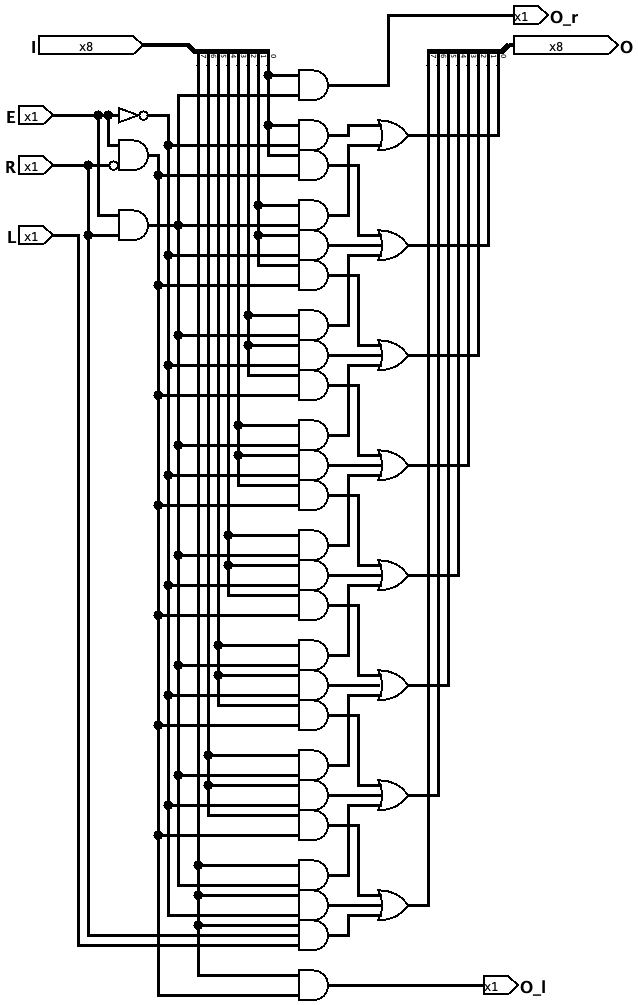
\includegraphics[scale=0.5]{Shiftre} \\
    \caption{Shiftre의 회로도}
    \label{fig:shr}
\end{figure}

\pagebreak

\subsection{OpCodeToFlags}

OpCodeToFlags는 4비트 연산자 코드를 ArithmetricLogic 플래그로 변환해주는
부품이다.

OpCodeToFlags는 $O_c$의 입력 핀과
$I_A$, $I_B$, $I_O$, $B_e$, $N$, $X$, $C_i$, $E$, $R$, $L$ 출력 핀을 가지고 있다.
$I_A$, $I_B$, $I_O$, $B_e$, $N$, $X$, $C_i$는 ArithmetricLogic에 입력되는 핀이고
$E$, $R$, $L$는 Shiftre에 입력되는 핀이다.

OpCodeToFlags의 진리표는 \tablename{} \ref{tab:octf}과 같다.

\begin{table}
    \centering
    \begin{tabular}{cl||ccccccc|ccc}
        $O_c$ & 연산자 & $I_A$ & $I_B$ & $I_O$ & $B_e$ & $N$ & $X$ & $C_i$ & $E$ & $R$ & $L$ \\
        \hline
        \texttt{0} & A    & 0 & 0 & 0 & 0 & - & - & 0 & 0 & - & - \\
        \texttt{1} & NOT  & 1 & 0 & 0 & 0 & - & - & 0 & 0 & - & - \\
        \texttt{2} & NEG  & 1 & 0 & 0 & 0 & - & - & 1 & 0 & - & - \\
        \texttt{3} & SHL  & 0 & 0 & 0 & 0 & - & - & 0 & 1 & 0 & - \\
        \texttt{4} & INC  & 0 & 0 & 0 & 0 & - & - & 1 & 0 & - & - \\
        \texttt{5} & DEC  & 0 & 1 & 0 & 1 & 0 & 0 & 0 & 0 & - & - \\
        \texttt{6} & ADD  & 0 & 0 & 0 & 1 & 0 & 0 & 0 & 0 & - & - \\
        \texttt{7} & SUB  & 0 & 1 & 0 & 0 & 0 & 0 & 1 & 0 & - & - \\
        \texttt{8} & XOR  & 0 & 0 & 0 & 1 & 0 & 1 & 0 & 0 & - & - \\
        \texttt{9} & XNOR & 0 & 0 & 1 & 1 & 0 & 1 & 0 & 0 & - & - \\
        \texttt{A} & AND  & 0 & 0 & 0 & 1 & 1 & 0 & 0 & 0 & - & - \\
        \texttt{B} & NAND & 0 & 0 & 1 & 1 & 1 & 0 & 0 & 0 & - & - \\
        \texttt{C} & OR   & 1 & 1 & 1 & 0 & 1 & 0 & 0 & 0 & - & - \\
        \texttt{D} & NOR  & 1 & 1 & 0 & 0 & 1 & 0 & 0 & 0 & - & - \\
        \texttt{E} & ASR  & 0 & 0 & 0 & 0 & - & - & 0 & 1 & 1 & 0 \\
        \texttt{F} & ASR  & 0 & 0 & 0 & 0 & - & - & 0 & 1 & 1 & 1 \\
    \end{tabular}
    \caption{OpCodeToFlags의 진리표}
    \label{tab:octf}
\end{table}

\begin{figure}[p]
    \centering
    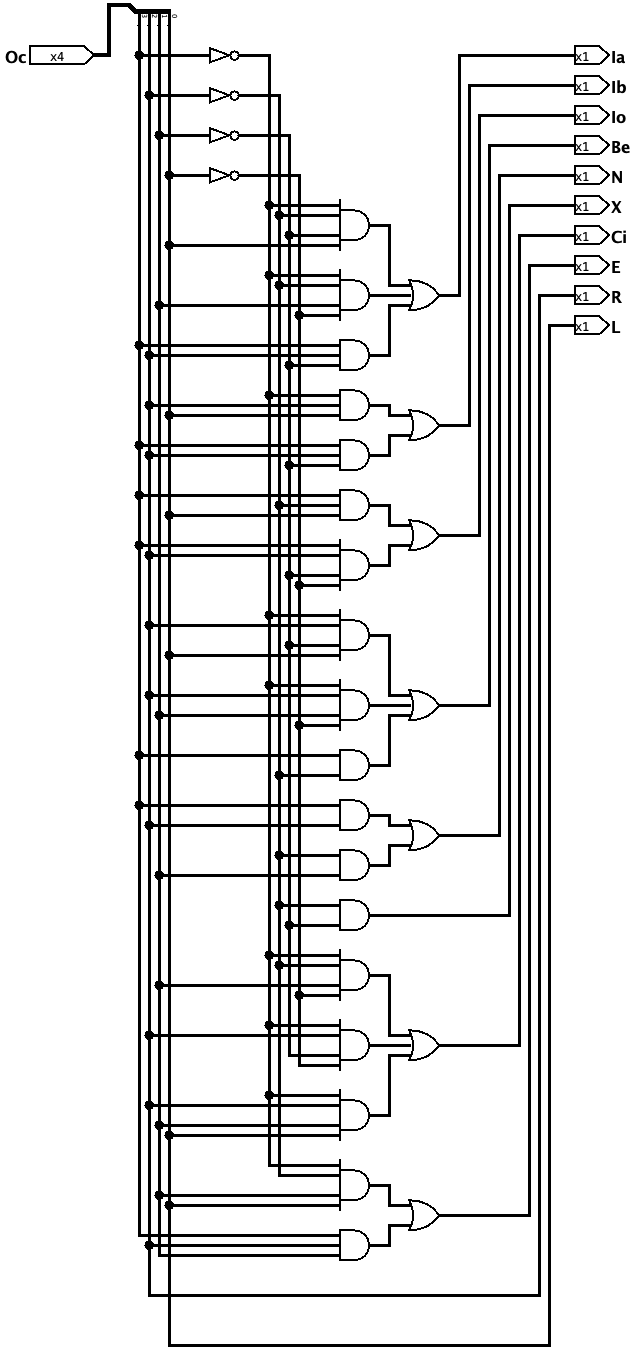
\includegraphics[scale=0.35]{OpCodeToFlags} \\
    \caption{OpCodeToFlags의 회로도}
    \label{fig:octf}
\end{figure}

\end{document}
